\section{Systematics Evaluation}
\subsection{1TS vs. 2TS}
The very first systematic study we did was to compare the results between 2
firmware configurations. All of HFM towers and half of HFP were sourced twice,
using either 1TS (with Operating Voltage 1) or 2TS (using Operating Voltage 2),
which provides us a measure of consistency in computing the calibration
coefficient across different firmware versions and operating voltages.
To compare these 2 modes of operation, we used ${CC}^{Run II}_{c}$ computed for
each sourcing configuration, after applying all the required corrections. The
distributions of ratios (1TS over 2TS) is presented in the Figures~\ref{fig:HF_1TSto2TS}.
Comparing 1TS OV1 and 2TS OV1+100 results, the source signals computed need to be corrected
for the 25\unit{ns} vs. 50\unit{ns} integration window. After correcting between the firmware
gains, the results agree to an order of 1\%.

\begin{figure}[htb]
    \begin{center}
        \subfigure[]
        {
            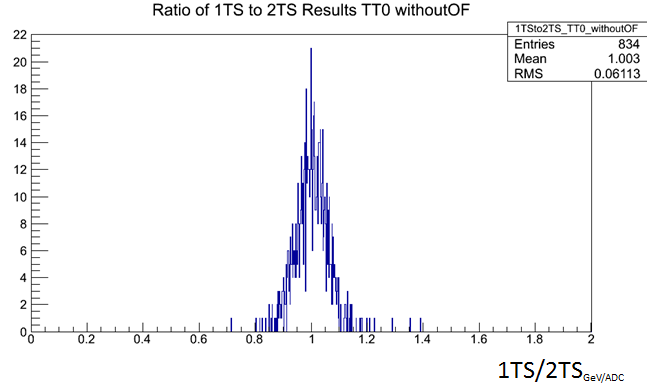
\includegraphics[width=.5\textwidth]{figures/ch_hfcalibration/HFM_1TSto2TS_woOF.png}
        }
        \subfigure[]
        {
            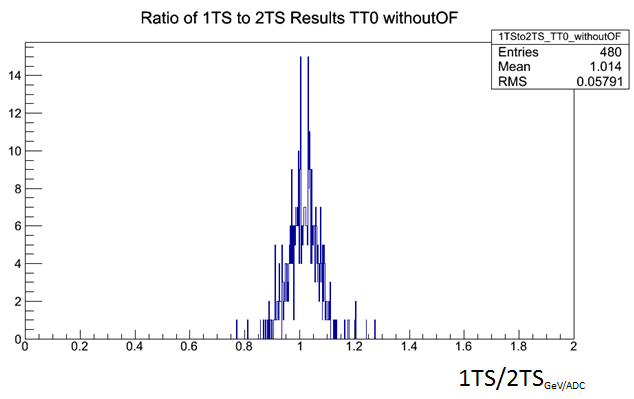
\includegraphics[width=.5\textwidth]{figures/ch_hfcalibration/HFP_1TSto2TS_woOF.png}
        }
        \caption
        {(a) Ratio of 1TS/2TS results for HFM.
         (b) Ratio of 1TS/2TS results for HFP
         For both sides The compared quantity was ${CC}^{Run II}_{c}$}
        \label{fig:HF_1TSto2TS}
    \end{center}
\end{figure}

As observed in the Figures~\ref{fig:HF_1TSto2TS},
1TS and 2TS results match both for HFP (1.4\%) and HFM (0.3\%) on the order of
under 1.5\%, which establishes solid indpendence of calibration coefficients from
the firmware used.

\subsection{Transversal Uniformity: Tubes A vs. Tubes B}
Approximately a quarter of HF wedges contains a second sourcing tube, which
differ in the groove type and as a consequence in the location within a wedge.
By comparing the obtained calibration coefficients using sourcing data from both
tubes, we can extract information on the transversal uniformity (or non-uniformity if you prefer) of the signal
within a wedge. Again, as in the case of 1TS-2TS study, we were comparing the
actual ${CC}^{Run II}_{c}$. The ratios are presented in the Figure~\ref{fig:HF_A2B}.
Transversal uniformity between A and B tubes within towers containing them, which is a quarter
of the towers within a given wedge, show good agreement between results as well, differing by
under 1\%.

\begin{figure}[htb]
    \begin{center}
        \subfigure[]
        {
            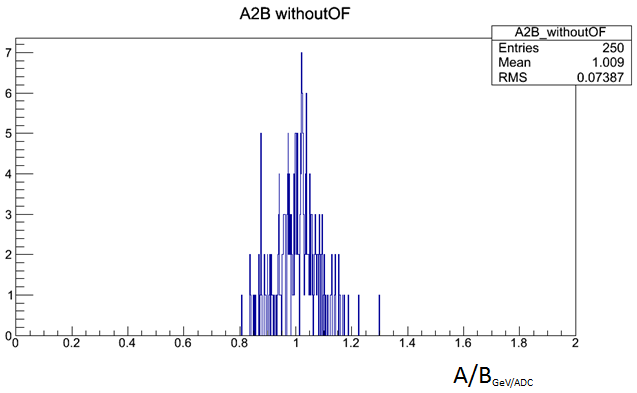
\includegraphics[width=.5\textwidth]{figures/ch_hfcalibration/HFM_A2B_woOF.png}
        }
        \subfigure[]
        {
            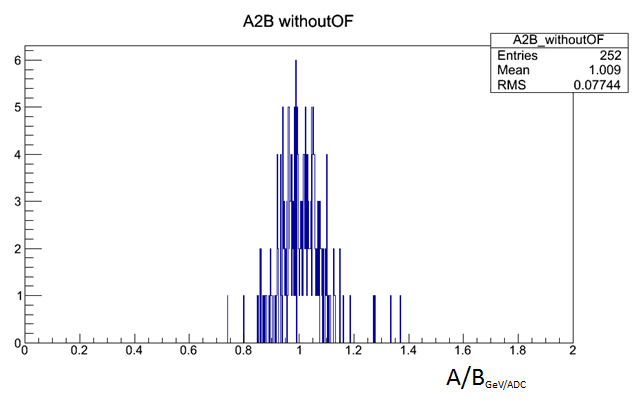
\includegraphics[width=.5\textwidth]{figures/ch_hfcalibration/HFP_A2B_woOF.png}
        }
        \caption
        {(a) Ratio of A/B results for HFM.
         (b) Ratio of A/B results for HFP
         For both sides The compared quantity was ${CC}^{Run II}_{c}$}
        \label{fig:HF_A2B}
    \end{center}
\end{figure}

As observed in the Figure~\ref{fig:HF_A2B}, on average the difference between
signals coming from A and B is on order of 1\%. The channel-to-channel variation
of the ratio is attributed to the Transversal Non-Uniformity of HF Wedges.

\subsection{Overflow Estimation}
Having the overflow bin is the major limitation of the DAQ system and the source of
systematic uncertainty for our analysis. As it was mentioned in the Experimental
Setup Section, both firmware types exhibit this behavior and even though 2TS
has a wider ADC range, the results will not differ dramatically from 1TS, because
differences in operating voltages will balance things out. However, in order to
provide some kind of "Lower Bound" error estimation for our charge measurement,
we separately computed calibration coefficients including the last bin in the
Eq.~\ref{eq:Histo_Avg} and compared them to the ones computed without. The results
for both HFM and HFP are presented in the Figure~\ref{fig:HF_Overflow}. Since we
do not know the actual adc counts in the overflow, when computing charge, we used
the center of the 32nd bin, as it was explained in the Experimental Setup section,
using which does provide us with "Lower Bound" estimation.

\begin{figure}[htb]
    \begin{center}
        \subfigure[]
        {
            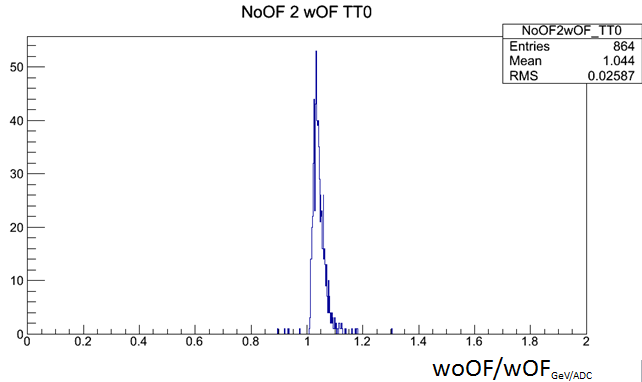
\includegraphics[width=.5\textwidth]{figures/ch_hfcalibration/HFM_NoOF2wOF_gevadc.png}
        }
        \subfigure[]
        {
            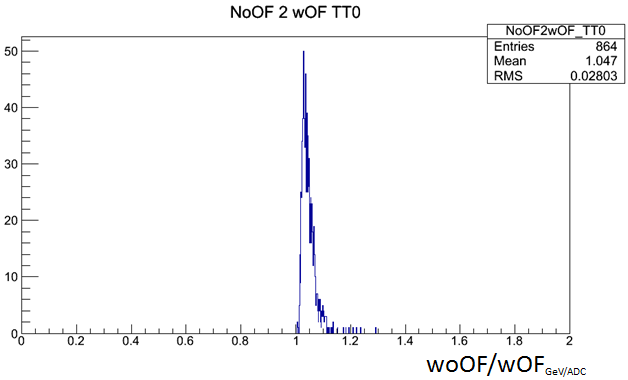
\includegraphics[width=.5\textwidth]{figures/ch_hfcalibration/HFP_NoOF2wOF_gevadc.png}
        }
        \caption
        {(a) Ratio of woOF/wOF results for HFM.
         (b) Ratio of woOF/wOF results for HFP
         For both sides The compared quantity was ${CC}^{Run II}_{c}$.
         Please note that the ratio appears to be $\geq1$ because the compared
         quantity isn't a signal, but rather an actual calibration coefficient,
         which contains energy over charge.}
        \label{fig:HF_Overflow}
    \end{center}
\end{figure}

As it can be observed in the Figure~\ref{fig:HF_Overflow}, the calibration
coefficients computed including the overflow bin introduce at least 4.4-4.7\%
difference into the measurement compared to the ${CC}^{Run II}_{c}$ computed
excluding overflow. These 4.4-4.7\% give us a lower bound on the amount of charge
that is approximately "sitting" in the overflow bin compared to the rest of the
ADC range. However, taking into consideration that we subtracted the pedestal
dynamically (inside the sum), we can notice that this is the amount of charge in
the overflow compared to the actual charge deposited by the radioactive source
(meaning that these charges are already pedestal-subtracted, which is very
important, considering that number of events in the pedestal dominate substantially).
Moreover, the actual number of events sitting in the overflow is under 1\% with
respect to the same ADC range. And considering that our integration window is
25\unit{ns} long, it is important to exclude for calibration purposes any
non-promptly originated signals.
It is also important to note that overflow contribution was excluded when analyzing 2013 sourcin campaign, as it didn't contain just overflow charge, but it also any event which was marked as a "hardware failure" went into the overflow bin.

\subsection{Longitudinal Uniformity}
As the radioactive source is moving along the source tube, we are actually able to
record the spatial information on the location of the source, which provides us
with yet another tool to estimate the uncertainty of our measurements. The general
idea is that we defined several regions along the source tube, summed up all the
histograms for each region respectively and then extracted the charges and
compared them.
As it was described in the Experimental Setup section, we have as an input all
the tubes' start (tubeStart) and end (tubeEnd) positions.
In the Table~\ref{tab:TubeRegions} we define the tubes' regions of interest to us.
"Front" and "Back" are defined so that "Front" is closer to IP and "Back" is further away.
"Signal" is the region that has been used as the defining region for extracting
the charge to be used in calibration coefficient calculation. And the "2/3Back"
is an additional region we defined to compare with the "Signal". It should be
noted that "2/3Back" and "Signal" have both overlapping and non-overlapping
regions. Even though overlapping region is the dominant one, using these 2 regions
we were trying to estimate how much the choice of the region influences the
actual charge computed.

From the Figure~\ref{fig:HF_LongUni}, we can observe that the signal in "Front" region is about 94-95\% of that compared to "Back" region. But we have to be more careful here when attributing this to systematics, as this mean ratio is consistent with the light attenuation in non-damaged fibers (due to light propogation). Therefore, this 5-6\% cannot be fully attributed to the systematics uncertainty. Considering the signal in "2/3Back" with respect to the "Signal" region, we observe a difference of 2\% on average, which is the the contribution to the systematic uncertainty due to the longitudinal non-uniformity of the signal.

\subsection{X-Checking}
An additional systematic uncertainty is included for the
methodology described in this note for measuring the absorber response to the source energy.
Independent analyses were performed on the same data, and the results were compared and agree
within an order of 1\%.

\begin{table}[!h] \centering \scalebox{1.10}{
    \begin{tabular}{|c|c|c|}
    \hline
    Region Name & Start & End \\
    \hline
    \hline
    Front(Depth 1 or EM) & tubeEnd-400 & tubeEnd-100 \\
    Front(Depth 2 or HAD) & tubeEnd-700 & tubeEdn-400 \\
    Back & tubeStart+100 & tubeStart+400 \\
    2/3Back & tubeStart & tubeStart+2/3(tubeEnd - tubeStart) \\
    Signal(EM and HAD) & tubeStart+300 & tubeEnd-300 \\
    \hline
    \end{tabular}}
    \caption{Source tube regions defined to provide a measure of uncertainty on
    the charge deposited in various regions along the source tube}
    \label{tab:TubeRegions}
\end{table}

\begin{figure}[htb]
    \begin{center}
        \subfigure[]
        {
            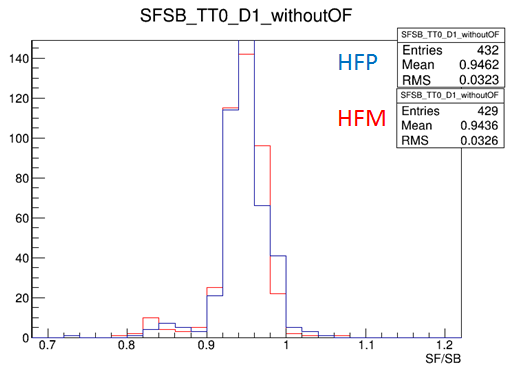
\includegraphics[width=.5\textwidth]{figures/ch_hfcalibration/SFSB_D1_woOF.png}
        }
        \subfigure[]
        {
            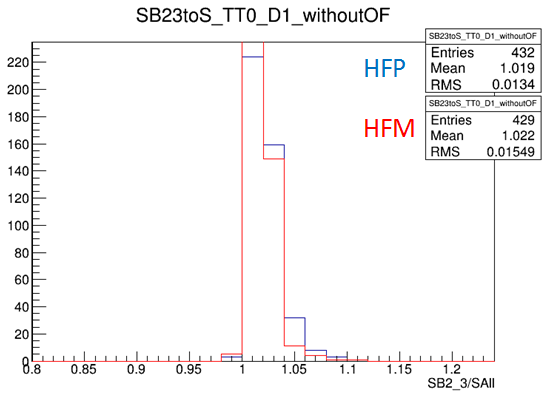
\includegraphics[width=.5\textwidth]{figures/ch_hfcalibration/SB23toS_D1_woOF.png}
        }
        \caption
        {(a) Ratio of the charge extracted from the "Front" region to the charge
         computed in the region "Back". Comparing Depth 1 or EM
         (b) Ratio of the charge computed within "2/3Back" region to the "Signal"
         region. Comparing Depth 1 or EM
         For both plots the compared quantity was the actual charge
         $Q$ADC/25\unit{ns}, excluding the overflow. Region are
         defined in the Table~\ref{tab:TubeRegions}}
        \label{fig:HF_LongUni}
    \end{center}
\end{figure}

\begin{figure}[htb]
    \begin{center}
        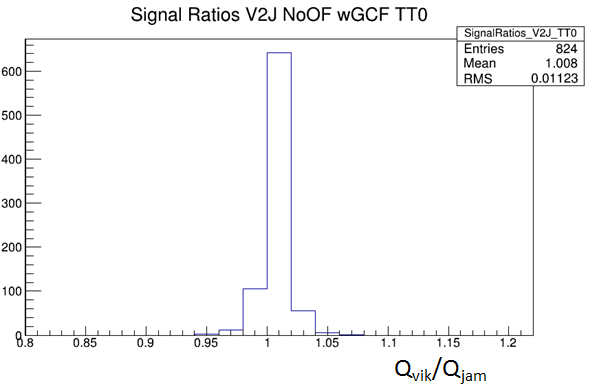
\includegraphics[width=.5\textwidth]{figures/ch_hfcalibration/Crosscheck.png}
        \caption{Cross-checking the results for HFM. On average the results agree
        within 1\%.}
        \label{fig:Crosscheck}
    \end{center}
\end{figure}
